\section{Decomposition method of MCT gate considering T-depth per bit}
In this chapter, we will explain the proposed method of decomposing MCT gate considering T-depth per bit.

\subsection{T-depth per bit}
In this section, we will explain T-depth per bit.

T-depth per bit is calculated for each quantum bit.

\par
We will explain how to calculate T-depth per bit.

Figure~\ref{toffoli_bit}
shows T-depth per bit of decomposition of Toffoli gate.

Let $q_{x}, q_{y}, q_{z}$ be the T-depth per bit of each input quantum bit.

First, the T-depth after execution of the $T$ gate on the left side of Figure~\ref{toffoli_bit}
is the T-depth per bit of that input plus 1.

The CNOT gates enclosed by the black solid lines in Figure~\ref{toffoli_bit}
cannot be executed until the input bits have been executed.
For this reason,
the bitwise T-depth after execution of the CNOT gates enclosed by the black solid lines can be considered to be the maximum bitwise T-depth of the input bits,
i.e., $\max\{q_{x}+1, q_{y}+1\}$.
If we consider the CNOT gates enclosed by the red dotted lines in the same way,
the bitwise T-depth after execution is $\max\{q_{x}+1, q_{y}+1, q_{z}+1\}$.
In this way,
if we calculate the bitwise T-depth from the left side of the Toffoli gate,
the bitwise T-depth after execution of the Toffoli gate can be considered to be $\max\{q_{x},q_{y},q_{z}\}+3$.
\begin{figure}
\centering
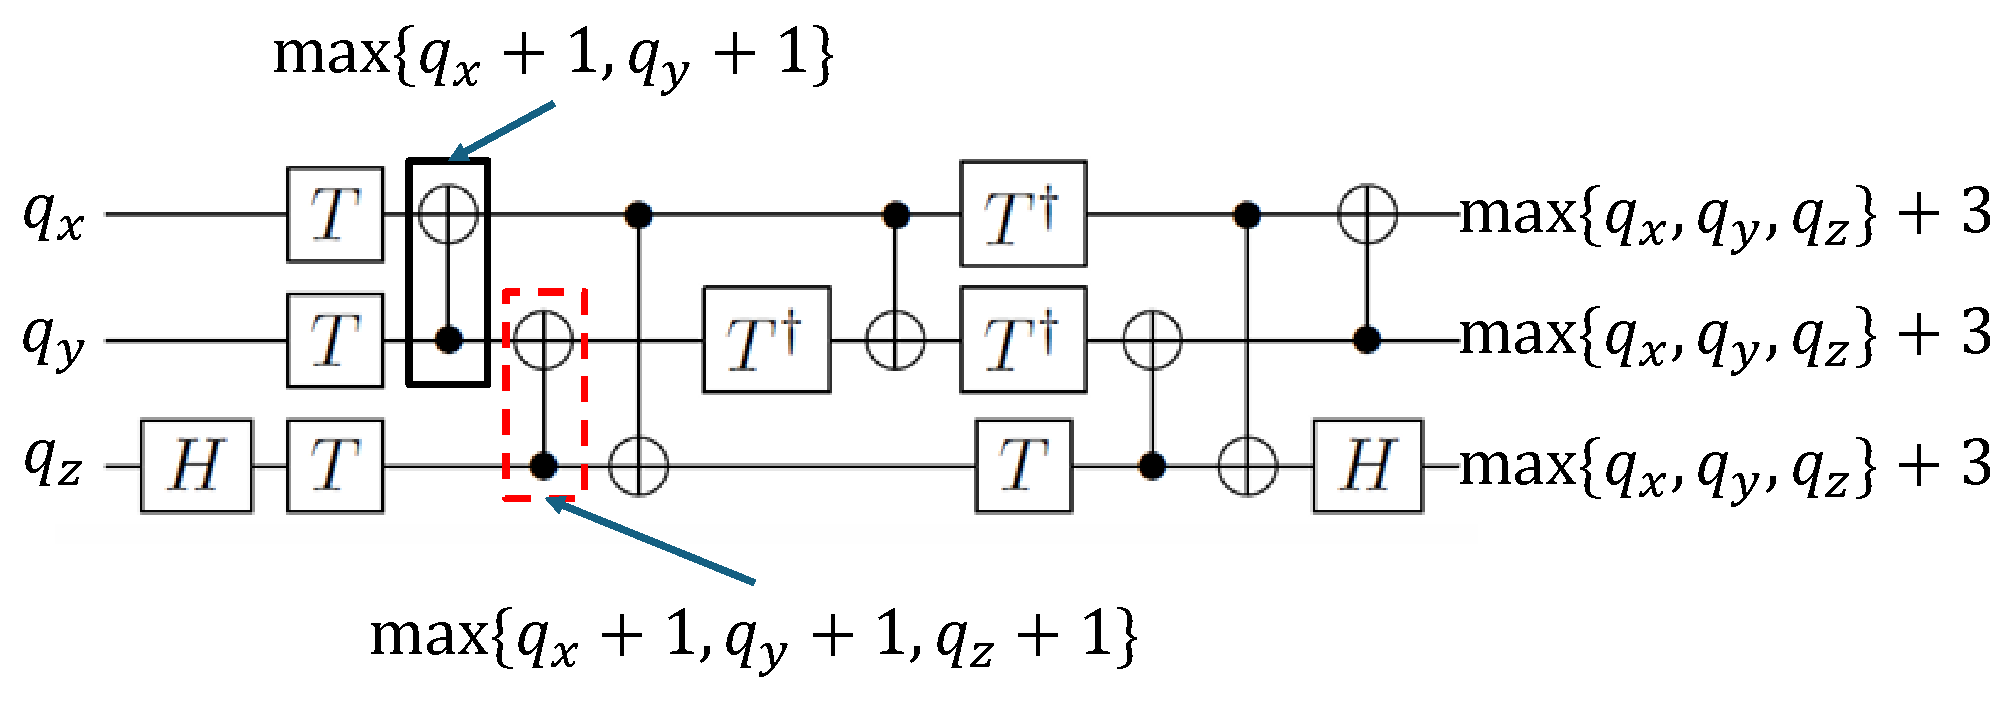
\includegraphics[width=12cm]{img/toffoli_bit.pdf}
\caption{T-depth per bit of Toffoli gate}
\label{toffoli_bit}
\end{figure}
\par
The T-depth per bit can be calculated from gates that can be decomposed into Clifford+T without using auxiliary bits.
Table~\ref{tab:gate_tdepth} shows the T-depth after executing gates that can be decomposed into Clifford+T without using auxiliary bits.
Based on Table~\ref{tab:gate_tdepth},
the T-depth per bit of the circuit can be obtained by calculating the T-depth per bit from the left side of the circuit.
\begin{table}[tbp]
\centering
\caption{T-depth after execution of gates that can be decomposed into Clifforf+T without using auxiliary bits}
\label{tab:gate_tdepth}
\begin{tabular}{c|cc}
Gate name &qubits used &T-depth after execution \\ \hline
$T, T^{\dag}$ &$q_{x} $ &$q_{x}+1$ \\
$H, NOT$ &$q_{x}$ &$q_{x}$ \\
$CNOT$ &$q_{x}, q_{y}$ &$\max\{q_{x}, q_{y}\}$ \\
\bout{Toffoli} &$q_{x}, q_{y}, q_{z}$&$\max\{q_{x},q_{y},q_{z}\}+3$\\ 
$CCiZ, CCiZ^{\dag} $&$q_{x}, q_{y}, q_{z}$&$\max\{q_{x},q_{y},q_{z}\}+2$\\
 $CCi\omega Z, CCi\omega Z^{\dag}$&$q_{x}, q_{y}, q_{z}$&$\max\{q_{x},q_{y},q_{z}\}+1$\\
 $C\omega S, C\omega S^{\dag}$ &$q_{x}, q_{y} $&$\max\{q_{x},q_{y}\}+1 $\\
 \end{tabular} \end{table}
\par
Figure~\ref{bit_tdepth} shows an example of calculating the T-depth for each bit based on Table~\ref{tab:gate_tdepth}.

The T-depth for each input bit in Figure~\ref{bit_tdepth} is all set to 0.

The maximum T-depth for Figure~\ref{bit_tdepth} is 12,
and the minimum T-depth is 8.

Figure~\ref{bit_tdepth} shows the T-depth for each bit obtained by decomposing an MCT gate with 4 control bits using Method~1.

When the T-depth for each bit is calculated in this way, there will be differences in the T-depth for each bit.

For this reason, by prioritizing bits with smaller T-depths

and decomposing the MCT gate, the T-depth for the entire circuit can be reduced.
\begin{figure}
\centering
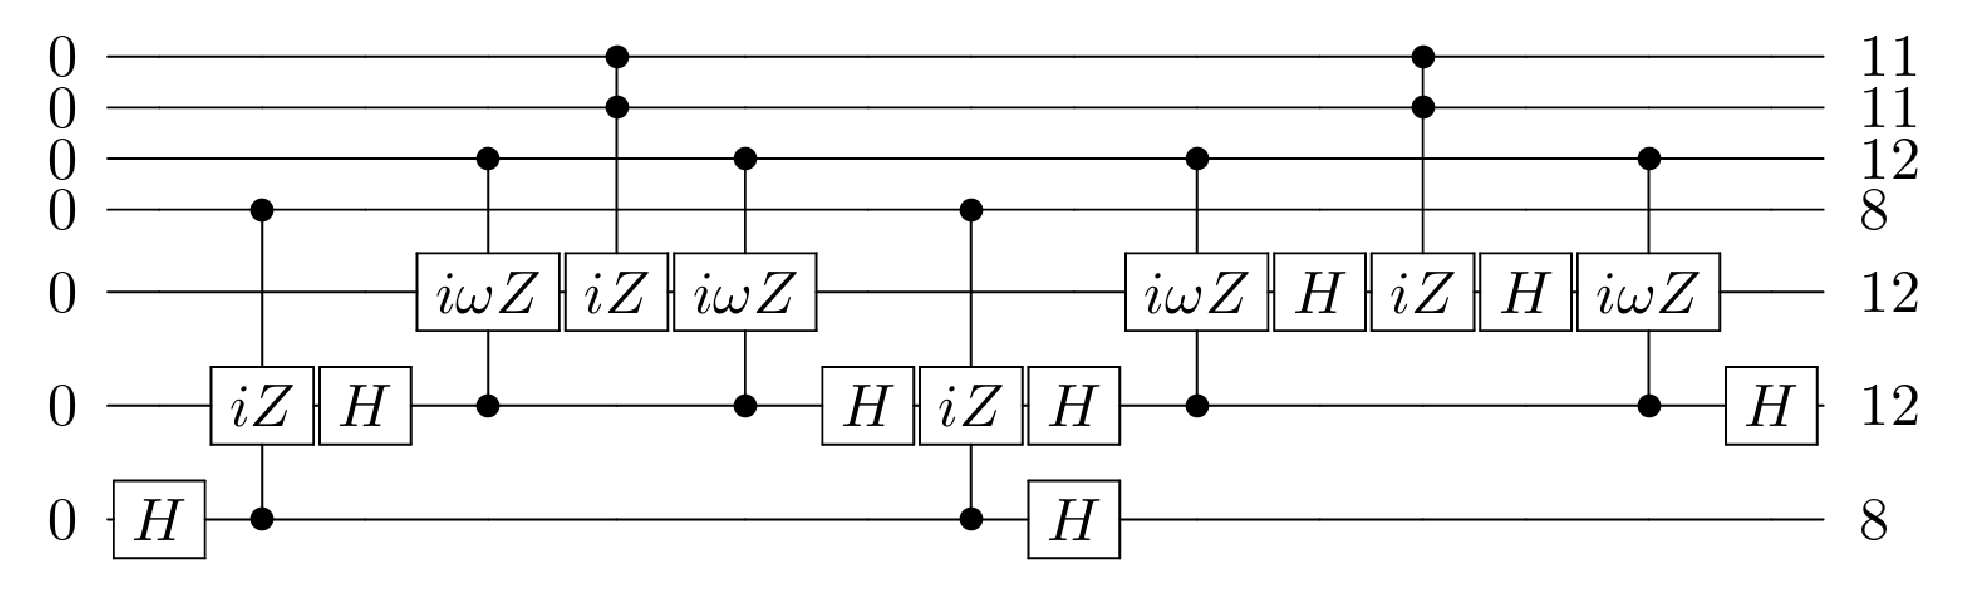
\includegraphics[width=14cm]{img/bit_tdepth.pdf}
\caption{T-depth per bit of the circuit in Figure~\ref{techmap}}
\label{bit_tdepth}
\end{figure}
\par
Figure~\ref{consider_tdepth} shows an example of decomposition of an MCT gate with three control bits, taking into account the T-depth per bit.
In Figure~\ref{consider_tdepth}, there is a difference in the T-depth of each bit on the input side.
Therefore, when applying decomposition that takes into account the T-depth of bits to method~1,
the T-depth can be reduced by using bits with the smallest T-depth in ascending order.
Figure~\ref{bad_consider_tdepth} shows an example in which the maximum T-depth after decomposition deteriorates due to bit selection.
In the example of Figure~\ref{bad_consider_tdepth},
if $q_{4}$ bits are used for the first gate $g_{1}$,
the maximum T-depth after execution of the \bout{subsequent} gates will be 20, since the T-depth depends on that value.
On the other hand, in Figure~\ref{consider_tdepth},
the maximum T-depth of the bits after decomposition is reduced by using the control bits and auxiliary bits in ascending order of T-depth.
\begin{figure}[tbp]
\centering
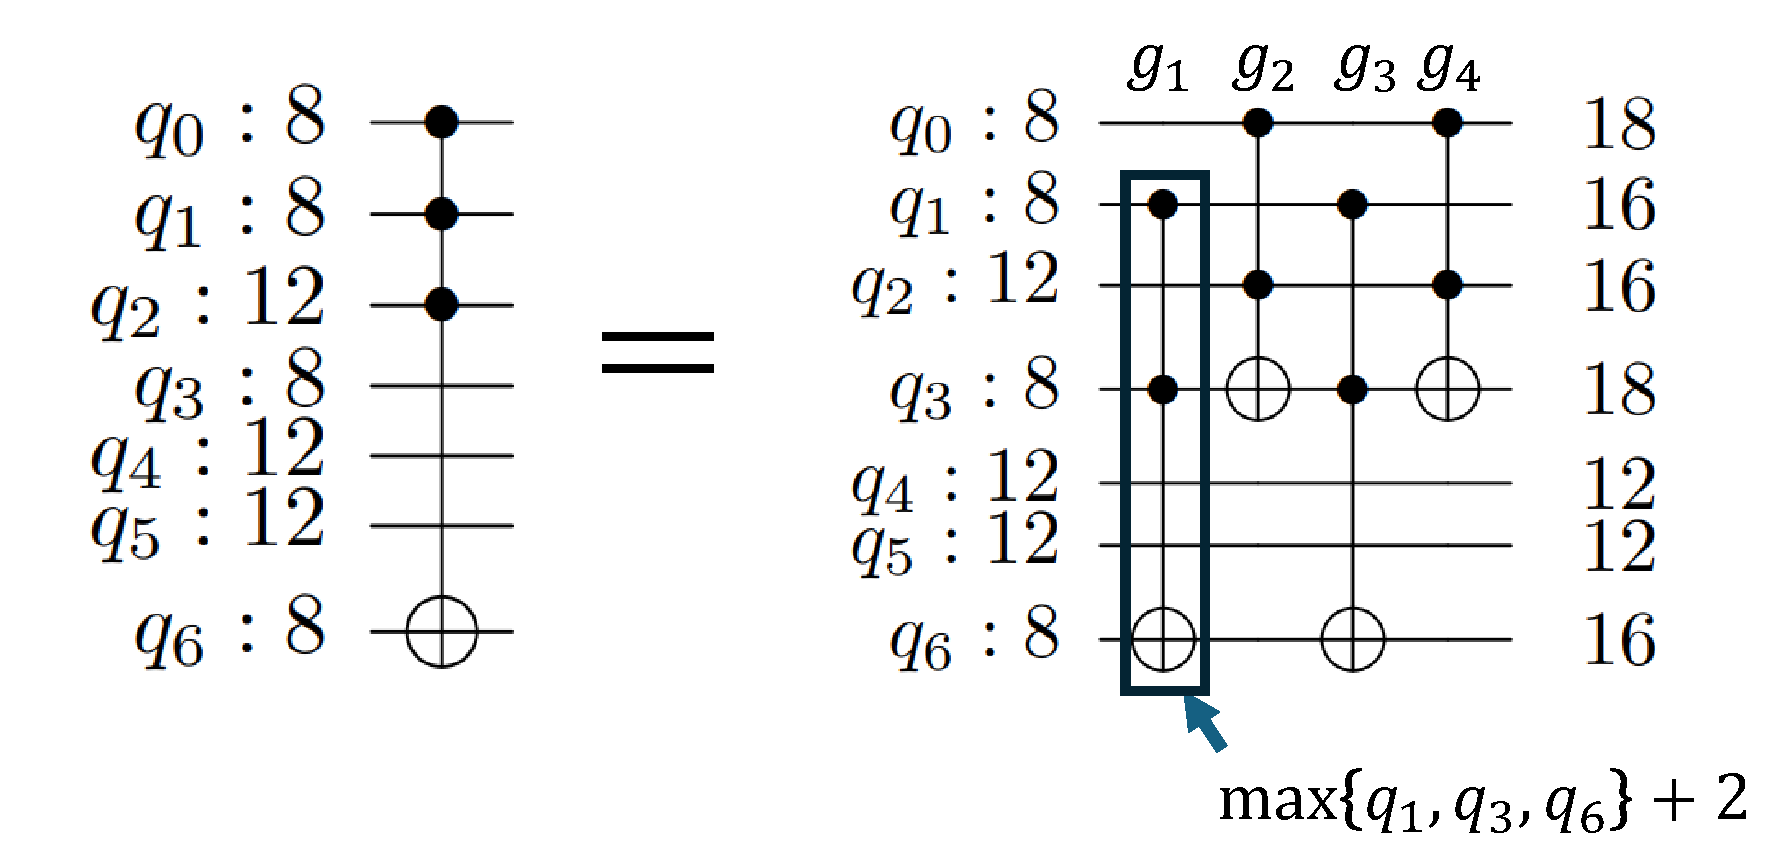
\includegraphics[width=10cm]{img/considering_bit_tdepth.pdf}
\caption{An example of decomposing an MCT gate with 3 control bits while considering the T-depth for each bit}
\label{consider_tdepth}
\end{figure}
\begin{figure}[tbp]
\centering
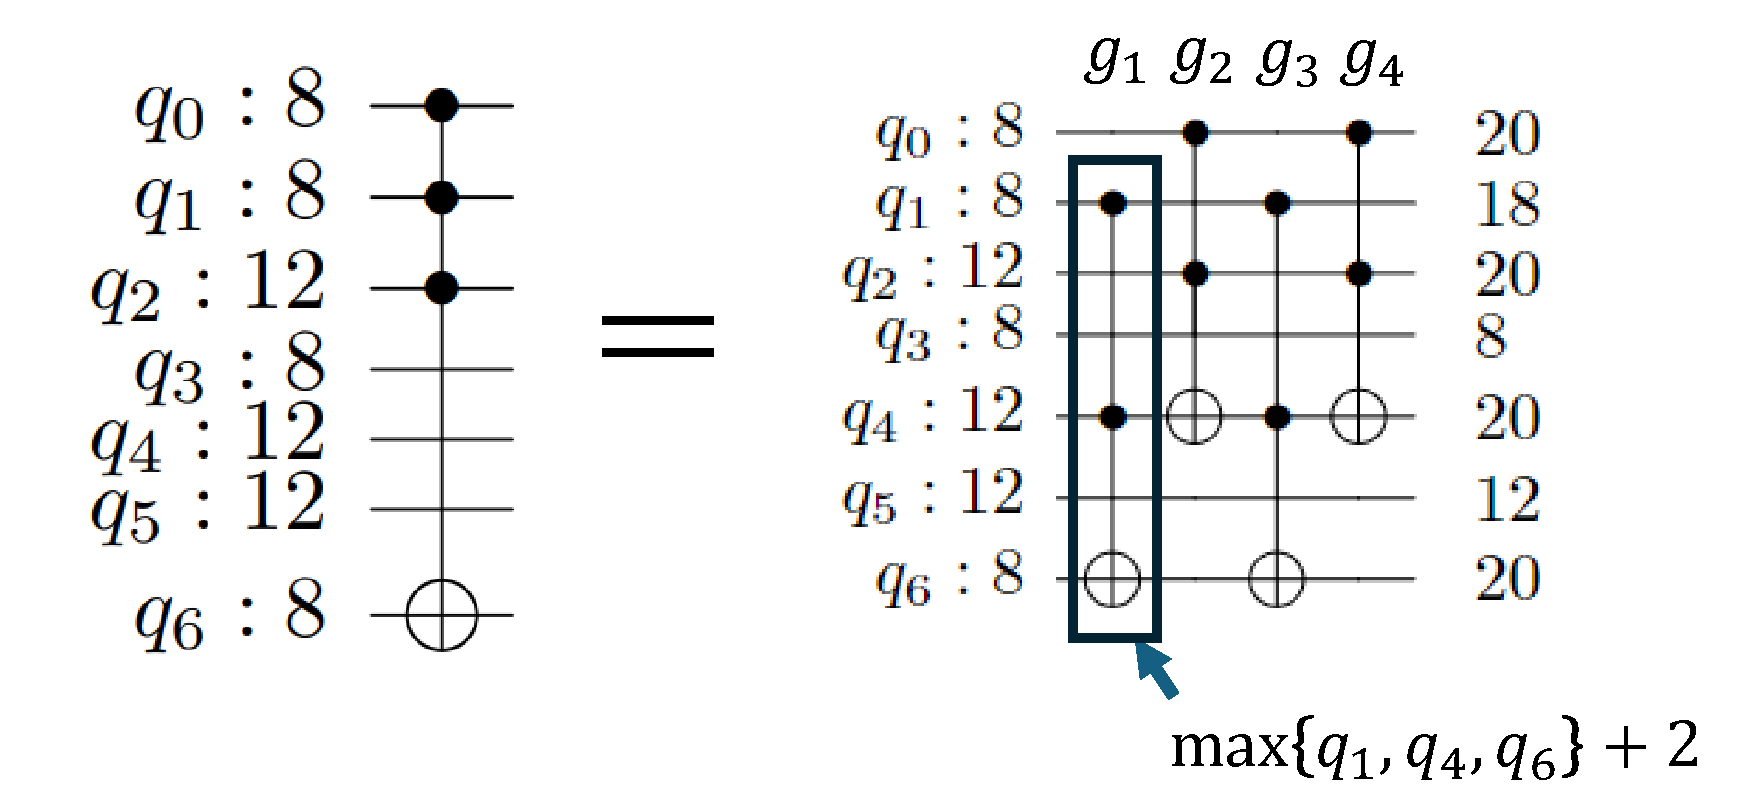
\includegraphics[width=10cm]{img/bad_consider_t-depth.pdf}
\caption{An example of the maximum T-depth deteriorating when decomposing an MCT gate with 3 control bits}
\label{bad_consider_tdepth}
\end{figure}
\subsection{Decomposing MCT gates while considering the T-depth for each bit}
In this section, we explain a method that applies methods 1 to 4 to decomposing MCT gates while considering the T-depth for each bit.
Here, $C$ is the set of $c$ control bits of the MCT gate before decomposition,
and $t$ is the target bit.
\subsection{Method~1}
In this section, we explain how to apply decomposition that considers the T-depth for each bit to Method~1.
\par
Method 1 is a method of decomposing an MCT gate with three or more control bits into a Toffoli gate,
and then replacing the Toffoli gate with a $CCiZ, CCi\omega Z$ gate.
Therefore, when decomposing an MCT gate into a Toffoli gate,
the arrangement of the gates is determined.
\par
We explain how to select bits when decomposing an MCT gate into a Toffoli gate.
Once the arrangement of the bits that make up the three Toffoli gates \rout{$g_{1},g_{2},g_{3}$}
from the left in Figure~\ref{barenco} is determined,
the decomposition of the MCT gate is determined, since the gates to the right are copies of these gates.
That is, in the method of decomposing an MCT gate using $c-2$ auxiliary bits with indefinite values~\cite{barenco1995elementary},
the decomposition can be achieved by determining the arrangement of $c-1$ Toffoli gates.
The method of determining the bits that compose these gates is explained below.
\par
Let $c_{1},\dots,c_{c}$ be the control bits of the MCT gate before decomposition
rearranged in ascending order of T-depth.
Let $t$ be the target bit of the MCT gate before decomposition.
Let $g_{1},\dots,g_{c-1}$ be the $c-1$ Toffoli gates from the left after decomposition.
Let $C_{1},\dots,C_{c-1}$ be the set of control bits of $g_{1},\dots,g_{c-1}$.
Let $a_{1},\dots,a_{c-2}$ be the $c-2$ auxiliary bits with indefinite values rearranged in ascending order of T-depth.
The method for determining the bits that make up $g_{1},\dots,g_{c-1}$ is shown below.
\begin{enumerate}[Step 1]
\item Add $a_{1},\dots,a_{c-2}$ one by one to $C_{1}\dots,C_{c-2}$ in order.
\item Add $c_{1},\dots,c_{c-2}$ to $C_{1},\dots,C_{c-2}$ in order.
\item Add $c_{c-1},c_{c}$ to $C_{c-1}$.
\item Let $t$ be the target bit of $g_{1}$.
\item Let $a_{1}, \dots, and a_{c-2}$ be the target bits of $g_{2}, \dots, and g_{c-2}$, in order.
\end{enumerate}
\par
After determining the bits that make up $g_{1}, \dots, and g_{c-1}$ according to the above procedure,

place the Toffoli gates from the left side of the circuit in the order of equation~\ref{eq:toffoli_haiti}.
\begin{equation}\label{eq:toffoli_haiti}
\{g_{1}, g_{2}, \dots g_{c-1}\},\{g_{c-2},g_{c-3},\dots g_{1}\}, \{g_{2},g_{3},\dots ,g_{c-1}\}, \{g_{c-2}, g_{c-3}\dots ,g_{2}\}
\end{equation}
Finally, these gates are replaced with $CCiZ, CCi\omega Z$ gates using method ~1.
In this way, by placing bits with smaller T-depth in order from the Toffoli gate on the left,
it is possible to prevent bits with larger T-depth from being used first.
\par
Figure ~\ref{b2mapping_proposed} shows an example of decomposing an MCT gate with 4 control bits using method ~1, taking into account the T-depth for each bit.
If the control bits of the MCT gate before decomposition on the left side of Figure~\ref{b2mapping_proposed} are rearranged in order of decreasing T-depth,

$C=\{c_{3}, c_{2}, c_{4}, c_{1}\}$.

The auxiliary bits with indefinite values have decreasing T-depth in the order of $a_{1}, a_{2}$.

First, determine the bits that make up $g_{1}, g_{2}, g_{3}$.

If the control bits of $g_{1}$ are selected in order of decreasing T-depth,

they become $c_{3}, a_{1}$,

and the target bit is $t$.

Next, if the control bits of $g_{2}$ are selected in order of decreasing T-depth,

they become $c_{2}, a_{2}$,

and the target bit is $a_{1}$.

Finally, the control bits of $g_{3}$ are $c_{4}, c_{1}$,
and the target bit is $a_{2}$.
In this way, the bits that make up $g_{1}, g_{2}, and g_{3}$ are determined,
and the Toffoli gates are placed in the order of equation~\ref{eq:toffoli_haiti}.
If the placed Toffoli gates are replaced with $CCiZ, CCi\omega Z$ gates using method~1,
it will look like the right side of Figure~\ref{b2mapping_proposed}. The maximum T-depth in this case is 24.
\begin{figure}
\centering
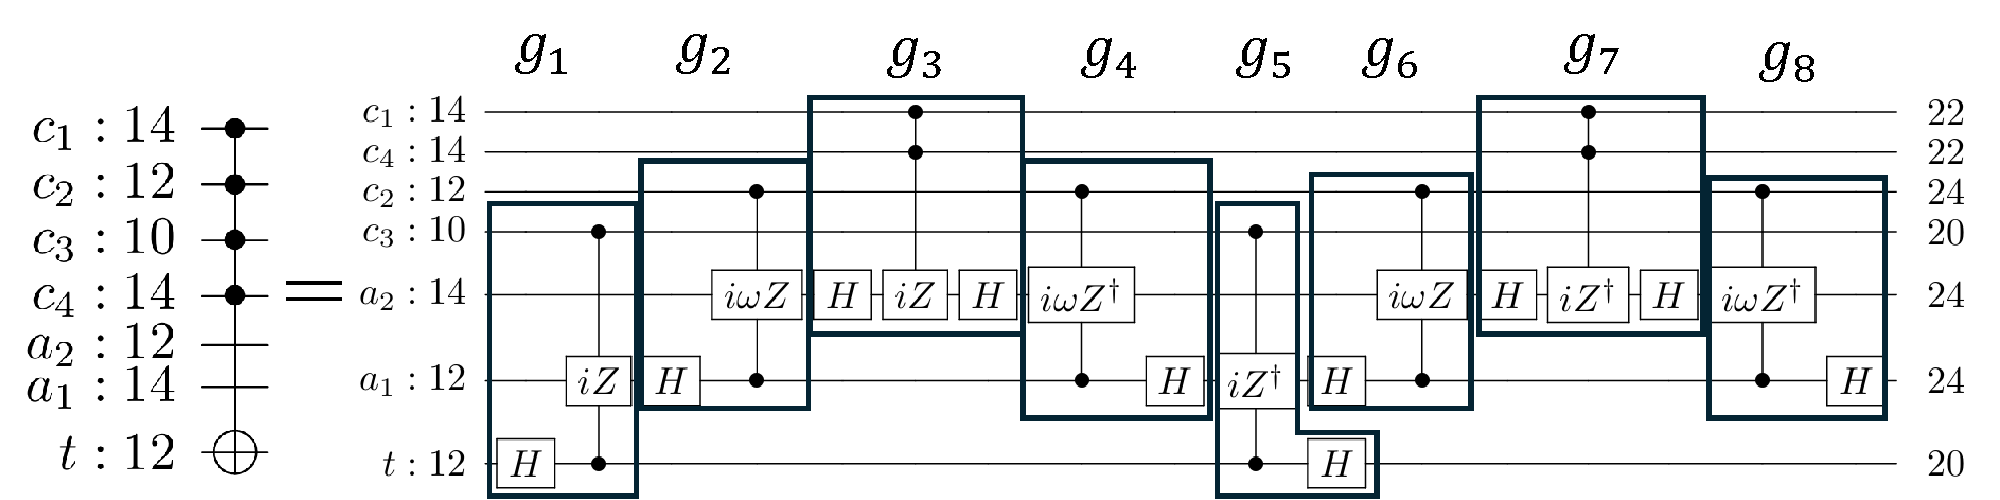
\includegraphics[width=18cm]{img/b2_mapping_proposed.pdf}
\caption{An example of decomposing an MCT gate with 4 control bits using method 1, taking into account the T-depth for each bit}
\label{b2mapping_proposed}
\end{figure}

\begin{comment}
\begin{algorithm}[tbp]
\caption{Decomposition taking into account the T-depth for each bit}\label{alg:b2map_bit}
\begin{algorithmic}[1]
\Require $tdepth\Leftarrow$ T-depth for each quantum bit
\Require $C\Leftarrow$ List of control bits for the MCT gate to be decomposed
\Require $t\Leftarrow$ Target bit for the MCT gate to be decomposed
\Require $D\Leftarrow$ List of uninitialized auxiliary bits
\Ensure $circ$: Decomposed MCT gate
\State $C \Leftarrow$ Sort the list of control bits in ascending order of T-depth
\State $D \Leftarrow$ Sort the list of auxiliary bits in ascending order of T-depth
\For{$(q,index) \leftarrow $C elements and their indexes}
\If{$i==0$}
\State
\EndIf
\EndFor
\end{algorithmic}
\end{algorithm}
\end{comment}
\subsection{Method 2}
In this section, we explain how to apply the decomposition that takes into account the T-depth of each bit to Method 2.
\par
In Method 2, the MCT gate is decomposed into four $C\omega S$ gates and four MCT gates.
First, we explain how to determine the bits that compose the four $C\omega S$ gates and four MCT gates that appear in the decomposition.
Let $a$ be a bit with an indefinite value.
First, the four $C\omega S$ gates have one undefined auxiliary bit $a$ as the control bit,
and $t$ as the target bit.
Next, the four MCT gates that appear in the decomposition are $g_{1},\dots, g_{4}$ from the left.
We will explain how to determine the bits that make up $g_{1} and g_{2}$.
The sets of control bits for $g_{1} and g_{2}$ are $C_{1} and C_{2}$.
The $c$ control bits of the MCT gates before decomposition
sorted in ascending order of T-depth are $c_{1},\dots, c_{c}$.
$C_{1} and C_{2}$ are determined according to the formula~\ref{eq:method2bunkatu}.
\begin{equation}\label{eq:method2bunkatu}
C_{1}=\{c_{1},\dots, c_{\lfloor c/2 \rfloor}\}, C_{2}=\{c_{\lfloor c/2 \rfloor +1},\dots , c_{c}\}
\end{equation}
The target bit of $g_{1} and g_{2}$ is $a$.
As for $g_{3} and g_{4}$, they are copies of $g_{1}$ and $g_{2}$, respectively,
so they are composed of the same bits as these gates.
In this way,
the bits that compose the four $C\omega S$ gates and four MCT gates that appear in the decomposition are determined.
\par
After determining the four $C\omega S$ gates and the bits that make up the four MCT gates that appear in the decomposition,
these gates are decomposed in order from the left, and the T-depth update for each bit is repeated.
These gates are decomposed and placed according to Algorithm~\ref{alg:method2_placement_decomp}.
In this way, by decomposing from the left gate,
each gate can be decomposed while taking into account the T-depth for each bit.
\begin{algorithm}[tbp]
\caption{Decomposition and placement of method 2 considering T-depth for each bit}
\label{alg:method2_placement_decomp}
\begin{algorithmic}[1]
\Require MCT gates $g_{1},\dots, g_{4}$
\Require $C\omega S$ gates
\Require Correspondence between each bit $c_{1},\dots, c_{c}, a, t$ and T-depth
\Ensure Circuit $OC$ consisting of gates that can be decomposed into Clifford+T without using auxiliary bits
\State $C_{i}$ is a set of control bits for $g_{i}$
\For{i={1,\dots ,2}}
\State $C\omega S$ gates are added to $OC$, and the T-depth for each bit is updated
\State $C_{(i+1)\% 2}$, extract $|C_{i}|-2$ bits in ascending order of T-depth.
\State Using the extracted $|C_{i}-2|$ bits as auxiliary bits, decompose $g_{i}$ using method ~1, taking into account the T-depth of each bit.
\State Add the decomposition result of $g_{i}$ to $OC$, and update the T-depth of each bit.
\EndFor
\For{i={1,\dots ,2}}
\State Add a $C\omega S$ gate to $OC$.
\State Add the decomposition of $g_{i}$ to $OC$ by replacing it with an inverse transformation gate and reversing the order.
\EndFor
\end{algorithmic}
\end{algorithm}
\par
\begin{figure}
\centering
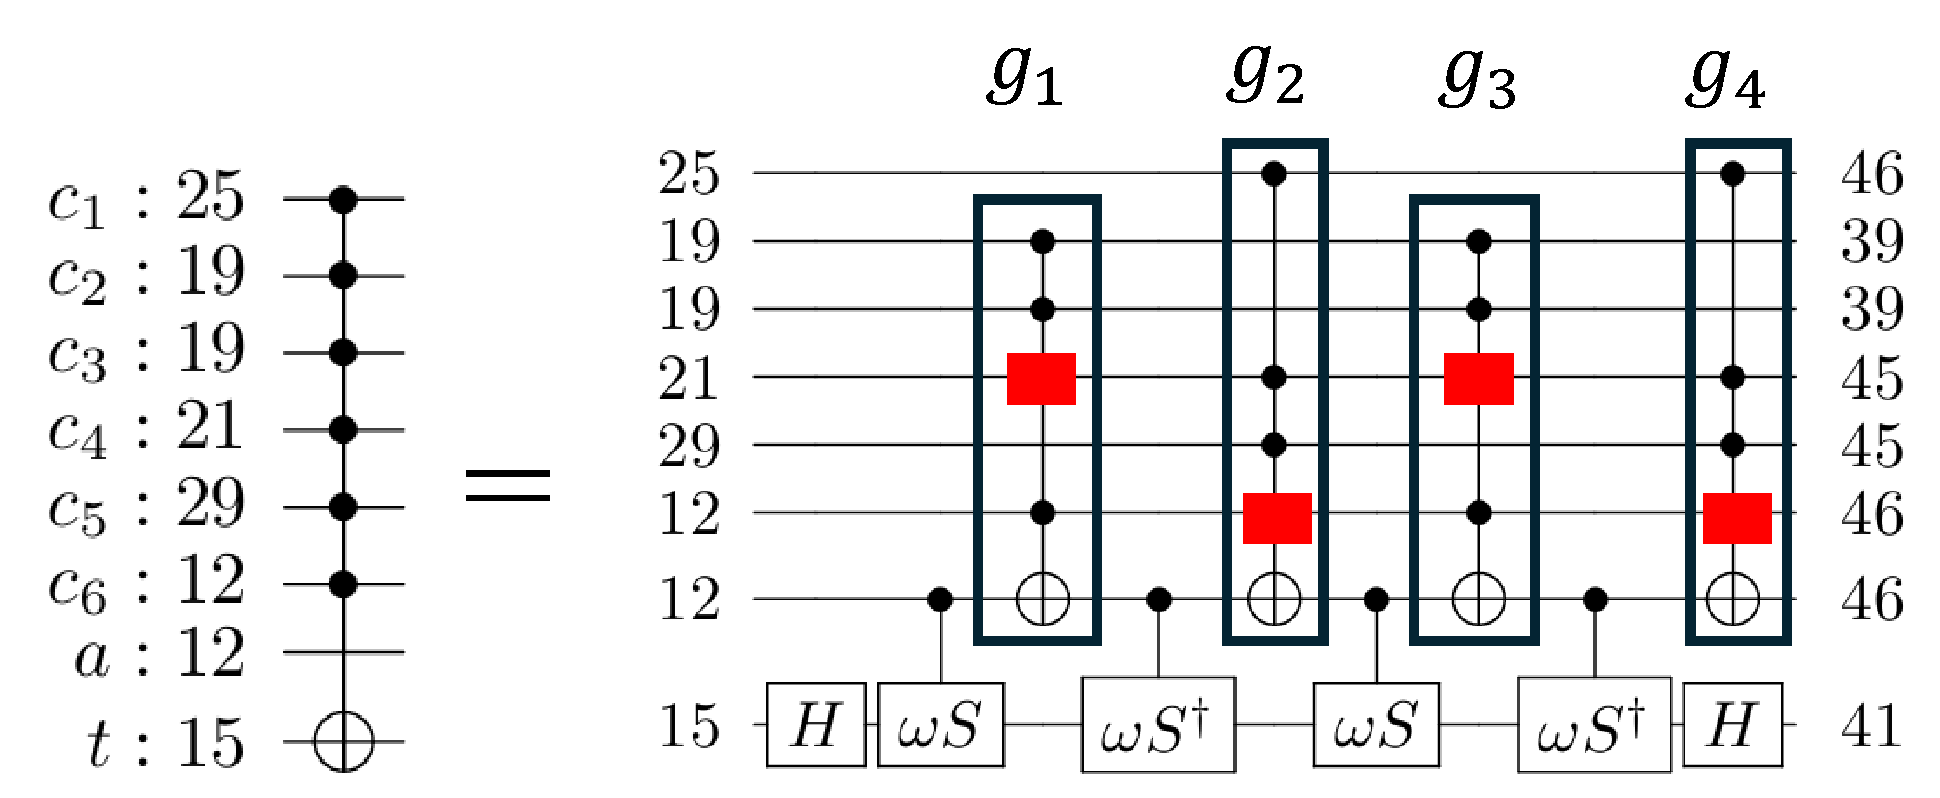
\includegraphics[width=10cm]{img/mimap_proposed.pdf}
\caption{An example of decomposing an MCT gate with 6 control bits using method ~2, taking into account the T-depth for each bit}
\label{mimap_proposed}
\end{figure}
\bout{Figure ~\ref{mimap_proposed} shows an example of decomposing an MCT gate with $c=6$ into four MCT gates and four $C\omega S$ gates using method ~2, taking into account the T-depth for each bit.
First, to decompose an MCT gate using method ~2, taking into account the T-depth for each bit,
divide the control bits into two sets in ascending order of T-depth according to equation ~\ref{eq:method2bunkatu}.
In the example of Figure~\ref{mimap_proposed}, $C_{1}=\{c_{6}, c_{2},c_{3}\}, C_{2}=\{c_{1}, c_{4}, c_{5}\}$.

Once the division of the control bits is determined,
the bits that make up the four MCT gates and the $C\omega S$ gate can be determined.

The right side of Figure~\ref{mimap_proposed} is an example of
the MCT gate with $c=6$ decomposed into four MCT gates and
four $C\omega S$ gates. }
\par
\bout{Finally, the gates in the circuit on the right side of Figure~\ref{mimap_proposed} are decomposed according to Algorithm~\ref{alg:method2_placement_decomp}

First, calculate the T-depth of each bit from the decomposition results of gates up to $g_{1}$,
and decompose $g_{1}$ using $c_{3}$ as an auxiliary bit.
Next, decompose $g_{2}$ using $c_{6}$ as an auxiliary bit from the decomposition results of gates up to $g_{2}$.
Finally, $g_{3}$ and $g_{4}$ are replaced with the inverse transformation of the decomposition of $g_{1}$ and $g_{2}$, respectively, and then arranged in reverse order.
By decomposing each gate in this way,
the maximum T-depth of the decomposition result of Figure~\ref{mimap_proposed} is 46. }
\subsection{Method 3}
We explain how to apply decomposition that takes into account the T-depth for each bit to Method~3.
\par
In method ~3, the number of control bits \rout{of each MCT gate after decomposition is determined according to the number of auxiliary bits $m\geq 2$ whose values are indefinite to be used in the decomposition and the number of control bits $c$ of the MCT gate to be decomposed. }
The number of control bits of each MCT gate $g_{1},\dots, g_{m+1}$ after decomposition obtained by method ~3 is set to $N_{1},\dots, N_{m+1}$.

In method ~3, the control bits are preferentially placed in the $1$th and $m+1$th gates, so the value of $N_{2},\dots, N_{m}$ is 2.

\par
First, to determine the decomposition of method ~3, it is necessary to determine the placement of $g_{1},\dots,g_{m+1}$.

However,However, if the number of control bits in $g_{1}$ is three or more, the T-depth of the bits used in $g_{2},\dots, g_{m+1}$ changes depending on the result of the decomposition of $g_{1}$.

Therefore, $g_{1}$ must be decomposed in advance taking into account the T-depth of each bit,
and then the placement of $g_{2},\dots, g_{m+1}$ must be determined depending on the result.

The set of control bits for $g_{1},\dots,g_{m+1}$ is defined as $C_{1},\dots,C_{m+1}$.

The set of $m$ indefinite bits used for the decomposition is defined as $A$.

The placement of $g_{1},\dots,g_{m+1}$ is determined according to the following procedure.
\begin{enumerate}[Step 1]
\item Determine the arrangement of $g_{1}$ and decompose it. Update the T-depth of each bit from the result of the decomposition.
\begin{enumerate}
\item Move the element with the smallest T-depth from $A$ to $C_{1}$.
\item Move elements from $C$ in ascending order of T-depth so that $|C_{1}|=N_{1}$.
\item Let $t_{1}=t$.
\item Select $|C_{1}|-2$ bits in ascending order of T-depth from among the bits that are not $C_{1}$ or $t$.
\item Using the selected bits as auxiliary bits, decompose $g_{1}$ using method ~1, taking into account the T-depth of each bit.
\item Update the T-depth of each bit from the result of the decomposition.
\end{enumerate}
\item Select and place bits from $g_{2}, \dots ,g_{m+1}$ in ascending order of T-depth.
\begin{enumerate}[(1)]
\item Let $i=2$.
\item Move the element of $A$ with the smallest T-depth to $C_{i}$.
\item Move elements from $C$ in ascending order of T-depth so that $|C_{i}|=N_{i}$.
\item Let $t_{i}$ be the element of $A$ moved to $g_{i-1}$.
\item As long as $i < m+1$, set $i=i+1$ and return to (2). Otherwise, exit.
\end{enumerate}
\end{enumerate}
The placement of $g_{1},\dots, and g_{m+1}$ is determined using this procedure.
After that,
according to Algorithm~\ref{alg:method3_placement_decomp},
we repeat the decomposition and bitwise T-depth updates,
and decompose and place the MCT gates in the order of formula~\ref{eq:bakerhaiti}.
\begin{algorithm}[tbp]
\caption{Placement and decomposition of method 3 considering T-depth for each bit}
\label{alg:method3_placement_decomp}
\begin{algorithmic}[1]
\Require List of MCT gates in formula ~\ref{eq:bakerhaiti}: $mctlist$
\Require Correspondence between each bit and T-depth
\Ensure Circuit composed of gates that can be decomposed into Clifford+T without using auxiliary bits: $OC$
\For{$g \leftarrow mctlist$}
\State Set of unused bits in \State $g$: $A$
\State Number of control bits in \State $g$: $c$
\State Extract $c-2$ bits from \State $A$ in ascending order of T-depth.
\State Using the extracted $c-2$ bits as auxiliary bits, $g$ is decomposed using method~1, taking into account the T-depth for each bit.
\State Add the decomposition result of $g$ to $OC$, and update the T-depth for each bit.
\EndFor
\end{algorithmic}
\end{algorithm}
\par
Figure~\ref{baker_proposed} shows an example of decomposing an MCT gate with $c=5$ using method~3, which takes into account the T-depth for each bit.
We will explain the decomposition of Figure~\ref{baker_proposed}.
First,
using method~3,
the number of control bits for each gate when decomposing the gate on the left side of Figure~\ref{baker_proposed} is calculated,
which is $N_{1}=3, N_{2}=2, N_{3}=2$.
Next, determine the bits that make up $g_{1}, g_{2}, g_{3}$ in order.
First, determine the control bit $C_{1}$ of $g_{1}$.

Of the auxiliary bits $a_{1}, a_{2}$, move the bit $a_{2}$ with the smallest T-depth to $C_{1}$.

Also, select two bits, $c_{2} and c_{5}$, from $c_{1},\dots,c_{5}$ in ascending order of T-depth value and move them to $C_{1}$.

Let $t$ be the target bit of $g_{1}$.

Since the number of control bits of $g_{1}$ is 3, the bits that make up the subsequent gates will change depending on the decomposition result of $g_{1}$.

Therefore, select $|C_{1}|-2$ bits in ascending order of T-depth from the bits not used by $g_{1}$, and decompose $g_{1}$.

In the example in Figure~\ref{baker_proposed}, $c_{3}$ is treated as an auxiliary bit, $g_{1}$ is decomposed, and the T-depth is recalculated.
After recalculation, the T-depth of each bit is $c_{2}=27, c_{3}=27, c_{5}=27, a_{2}=25, t=25$.
From this result, the bits that make up $g_{2} and g_{3}$ are determined.
The control bits of $g_{2}$ are $a_{1}$, and
of $c_{1}, c_{3}, and c_{4}$, $c_{1}$ is the bit with the smallest T-depth.
Additionally, the target bit of $g_{2}$ is $a_{2}$.
The control bits of $g_{3}$ are the remaining control bits $c_{3}, c_{4}$,
and the target bit is $a_{1}$.

In this way, the bits that make up $g_{1}, g_{2}, g_{3}$ are determined,
and the decomposition on the right side of Figure~\ref{baker_proposed} can be realized by arranging them in the order of equation~\ref{eq:bakerhaiti}.
\par
\bout{Finally, the gates $g_{1},\dots, g_{8}$ on the right side of Figure~\ref{baker_proposed}
are decomposed and arranged from the left side according to Algrorithm~\ref{alg:method3_placement_decomp},
and the decomposition of Method~3, which takes into account the T-depth for each bit, can be determined.

First, $g_{1}$ is decomposed using $c_{3}$, which has the smallest T-depth, as an auxiliary bit.

$g_{5}$ is decomposed using the smallest T-depth bit $c_{4}$ from the decomposition results of $g_{1},\dots, g_{4}$ as an auxiliary bit.
After decomposing all gates, the maximum T-depth is 41. }
\begin{figure}[tbp]
\centering
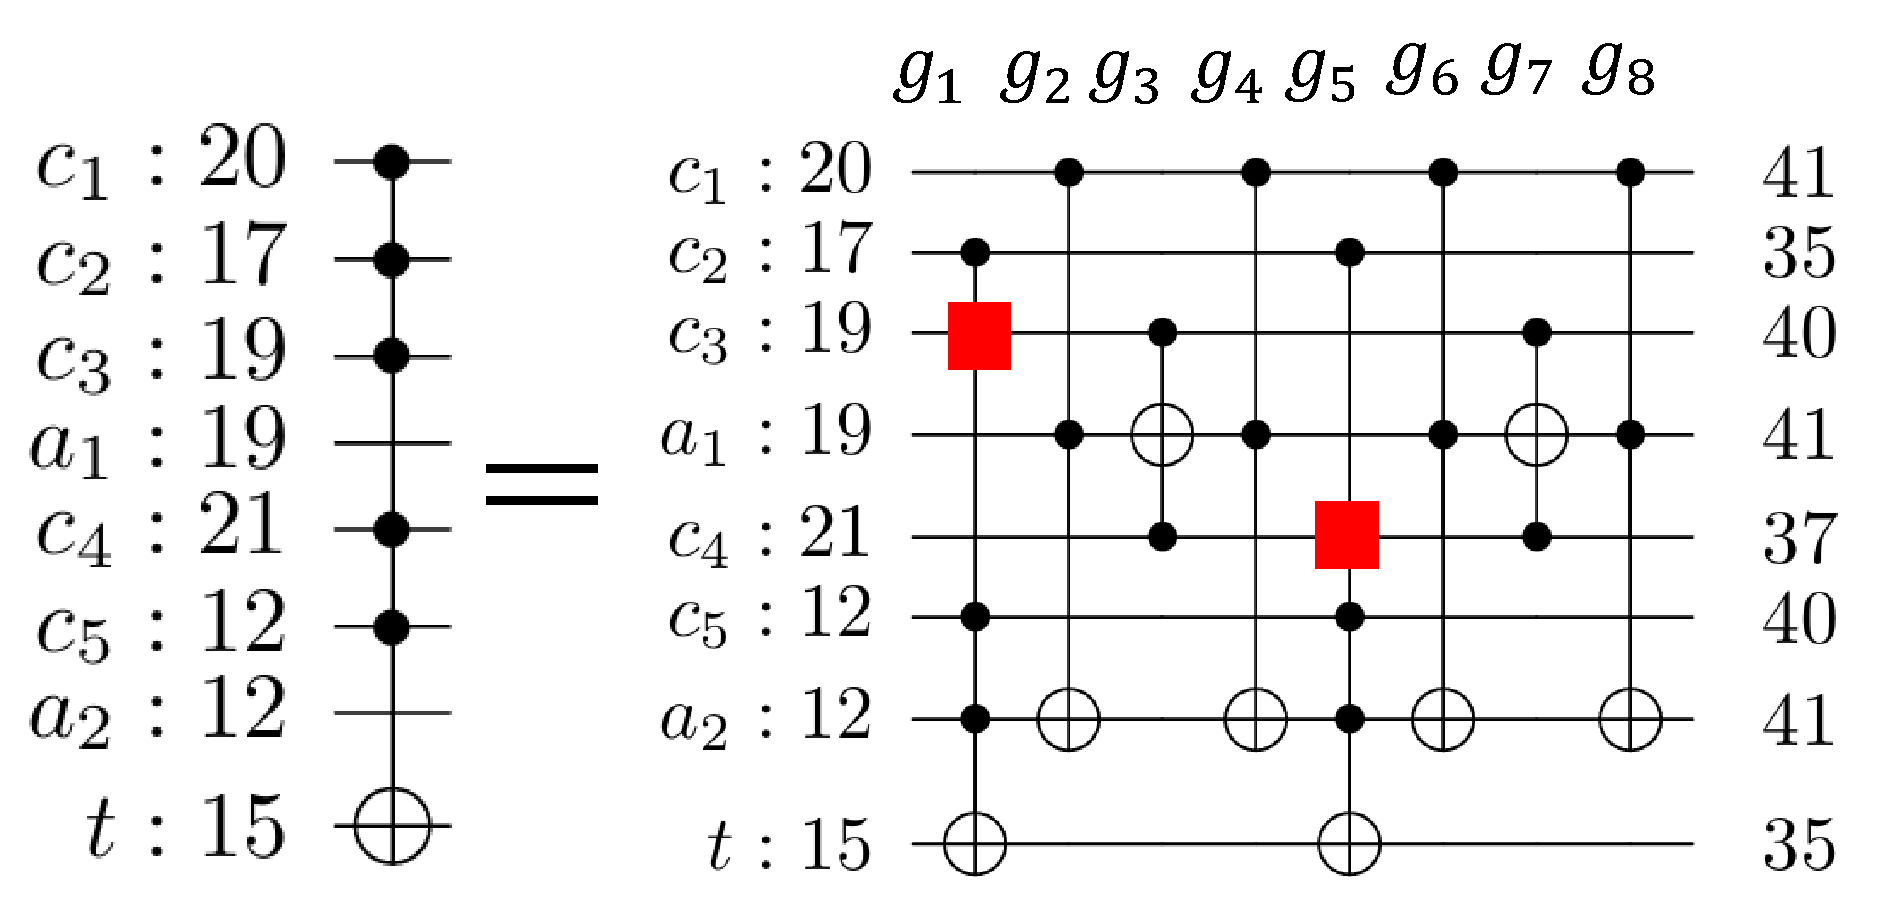
\includegraphics[width=10cm]{img/baker_proposed.pdf}
\caption{An example of decomposing an MCT gate with $c=5$ using method 3, taking into account the T-depth of each bit, with two auxiliary bits of indefinite value}
\label{baker_proposed}
\end{figure}
\begin{comment}
\begin{algorithm}[tbp]
\caption{Placement and decomposition of method 3, taking into account the T-depth of each bit}
\label{alg:method3_placement_decomp}
\begin{algorithmic}[1]
\Require MCT gate before decomposition $(C, t)$ \Comment{$C$ is a set of control bits, $t$ is a target bit}
\Require List of $m$ auxiliary bits $A$
\Require T-depth of each bit
\Ensure $OC$ is a circuit consisting of gates that can be decomposed into Clifford+T without using auxiliary bits.

\State List of empty bits $C_{1},\dots ,C_{m+1}$

\State $m+1$ bits $t_{1},\dots, t_{m+1}$

\State $t_{1} \leftarrow t$

\State $C_{1}$ adds the bit with the smallest T-depth in $A$

\State $t_{2} \leftarrow A$ the bit with the smallest T-depth

\State $A$ removes the bit with the smallest T-depth

\State $C \leftarrow$ Control bits of MCT gate before decomposition

\While{$|C_{1}|-2 \leq c+m-1$ and $|C|\geq m$}

\State $C_{1}$ adds the bit with the smallest T-depth in $C$

\State $C$ removes the bit with the smallest T-depth
\EndWhile
\State $g_{1}\leftarrow (C_{1}, t_{1})$
\State $g_{1}$ is decomposed using $|C_{1}|-2$ bits that are not part of $g_{1}$
\State $g_{1}$ decomposition is added to $OC$
\State $g_{1}$ decomposition is updated for each bit
\For{$i={2,\dots ,m}$}
\State $A$ element with minimum T-depth is added to $C_{i}$
\State $t_{i+1}\leftarrow A$ element with minimum T-depth
\State $A$ element with minimum T-depth is deleted
\State $C$ element with minimum T-depth is added to $C_{i}$
\State $C$ element with minimum T-depth is deleted
\State $g_{i}\leftarrow (C_{i}, t_{i})$
\State Replace $g_{i}$ with $CCi\omega Z$ gate

\State Add $g_{i}$ to $OC$

\EndFor

\State Update the T-depth of each bit

\State $C_{m+1} \leftarrow C$

\If{$|C_{m+1}|=2$}

\State Replace $g_{m+1}$ with $CCiZ$ gate

\State Add $g_{m+1}$ to $OC$

\Else

\State Among the bits that do not constitute $g_{m+1}$, extract $|C_{m+1}|-2$ bits in ascending order of T-depth.

\State Decompose $g_{m+1}$ by using the extracted bits as auxiliary bits, taking into account the T-depth of each bit

\EndIf

\end{algorithmic}
\end{algorithm}
\end{comment}
\subsection{Method 4}
We will explain how to decompose Method 4 by considering the T-depth for each bit.
\par
In Method 4, MCT gates are decomposed into multiple stages according to the number of auxiliary bits used in the decomposition.
The number of control bits for each decomposed MCT gate changes according to the number of auxiliary bits used and the number of control bits for the MCT gate to be decomposed.
The number of auxiliary bits with indefinite values used in the decomposition is $d$, and the number of auxiliary bits with a value of 0 used in the decomposition is $k$.
The number of control bits for the MCT gates in each stage can be calculated from Method 4 using these $c, k, and d$ values.
When MCT gates are decomposed using Method 4, it is assumed that they can be decomposed into $n$ stages. In this case, $n$ is an odd number equal to or greater than 3.
The number of control bits for the MCT gates in each stage is expressed using a two-dimensional array as shown in the formula~\ref{eq:niemann_cnt}.
In equation~\ref{eq:niemann_cnt},
of the gates in the $n$th stage, the MCT gates in the $\lceil \frac{n}{2} \rceil+1$th stage and beyond are omitted because they are copies of the gates in the first stage to the $\lceil \frac{n}{2} \rceil -1$th stage.
The subscript $N$ indicates the stage number and the MCT gate number.
For example, $N_{i, j}$ indicates the number of control bits of the $j$th MCT gate in the $i$th stage.
The $\lceil \frac{n}{2} \rceil$th stage is the central stage, so there is only one gate in this stage.
Therefore, $m_{\lceil \frac{n}{2} \rceil}=1$.
\begin{equation}\label{eq:niemann_cnt}
 \begin{pmatrix}
 N_{1,1} & N_{1,2} & \dots & N_{1,m_{1}} \\
 N_{2,1} & N_{2,2} & \dots & N_{2,m_{2}} \\
 \vdots & \vdots & \ddots & \vdots \\
 N_{\lceil \frac{n}{2} \rceil,1} & N_{\lceil \frac{n}{2} \rceil,2} & \dots & N_{\lceil \frac{n}{2} \rceil,m_{\lceil \frac{n}{2} \rceil}} \end{pmatrix}
\end{equation}
Using this formula~\ref{eq:niemann_cnt}, the number of control bits for each stage of the decomposition in Figure~\ref{niemann_c_2} is shown in
formula~\ref{eq:niemann_c_2}.
\begin{equation}\label{eq:niemann_c_2}
\begin{pmatrix}
2 & 2 & 2 & 2 \\
2 & 2 & & \\
2 & & & \\
2 & & & \\
\end{pmatrix}
\end{equation}
\par
In the proposed method, the placement and decomposition of the MCT gates after decomposition are determined according to the number of control bits for the MCT gates at each stage obtained by method~4.
The set of $k$ auxiliary bits with a value of 0 that can be used for decomposition is called $CA$.
The bits that make up the MCT gate at $\lceil \frac{n}{2} \rceil$ stage are determined by the following procedure.
\begin{enumerate}[Step 1]
\item Let $i=1$.
\item Prepare empty sets $C_{1},\dots ,C_{m_{i}}$. Let $j=1$.
\item Move elements from $C$ in ascending order of T-depth so that $|C_{j}|=N_{i, j}$.
\item If $j<m_{i}$, set $j=j+1$ and return to step 3.
\item Move the bits with the smallest T-depth of $CA$ to $t_{1},\dots, t_{m_{i}}$ one by one in order.
\item Let $C_{1},\dots, C_{m_{i}}$ be the control bits of gate $g_{i, 1},\dots, g_{i, m_{i}}$, and $t_{1},\dots ,t_{m_{i}}$ be the target bits.
\item Find the set $A$ of unused bits in $g_{i, 1},\dots ,g_{i, m_{i}}$.
\item Let $k=1$.
\item To avoid using the same auxiliary bits,
select $|C_{m_{k}}-2|$ auxiliary bits from $A$ in ascending order of T-depth, and delete those elements from $A$.
\item Using the selected auxiliary bits,
decompose $g_{i, k}$ using method 1,
taking into account the T-depth for each bit.
\item If $k < m_{i}$, set $k=k+1$ and return to step 9. Otherwise, proceed to the next step.
\item Update the T-depth of each bit.
\item Add $t_{1},\dots, t_{m_{i}}$ to $C$.
\item If $i< \lceil \frac{n}{2} \rceil$, set $i=i+1$ and return to step 2.
\item Let $C$ be the control bit of the MCT gate $g_{\lceil \frac{n}{2} \rceil, 1}$, and $t$ be the target bit.
\end{enumerate}
The above steps determine the bits that make up the MCT gate at the $1,\dots ,\lceil \frac{n}{2} \rceil$ stage.
The MCT gates at each stage that determine the constituent bits have information, including duplication, in the form of equation~\ref{eq:niemann_gates}.
\begin{equation}\label{eq:niemann_gates}
 \begin{pmatrix}
 g_{1,1} & g_{1,2} & \dots & g_{1,m_{1}} \\
 g_{2,1} & g_{2,2} & \dots & g_{2,m_{2}} \\
 \vdots & \vdots & \ddots & \vdots \\
 g_{\lceil \frac{n}{2} \rceil,1} & g_{\lceil \frac{n}{2} \rceil,2} & \dots & g_{\lceil \frac{n}{2} \rceil,m_{\lceil \frac{n}{2} \rceil}}\\
 g_{\lceil \frac{n}{2} \rceil -1, 1} & g_{\lceil \frac{n}{2} \rceil-1 ,2}& \dots & g_{\lceil \frac{n}{2} \rceil-1 ,m_{\lceil \frac{n}{2} \rceil-1}}\\
\vdots & \vdots & \ddots &\vdots \\
g_{1,1} & g_{1,2} & \dots & g_{1,m_{1}} \\
\end{pmatrix}
\end{equation}
\par
The decomposition of method 4 can be determined by decomposing the MCT gates in
formula~\ref{eq:niemann_gates},
which determine the constituent bits, using method 1,
taking into account the T-depth for each bit.
According to Algorithm~\ref{alg:method4_placement_decomp},
we repeatedly decompose and place the MCT gates in
the formula~\ref{eq:niemann_gates} to determine the decomposition.
\begin{algorithm}[tbp]
\caption{Decomposition and placement of method 4 considering T-depth for each bit}
\label{alg:method4_placement_decomp}
\begin{algorithmic}[1]
\Require 2D array of MCT gates in formula ~\ref{eq:niemann_gates}: $mctlist$
\Require Correspondence between each bit and T-depth
\Ensure Circuit composed of gates that can be decomposed into Clifford+T without using auxiliary bits: $OC$
\For{$pqgate \leftarrow mctlist$}
\State Set of bits not used in $pqgate$: $A$
\For{$g\leftarrow pqgate$}
\State Number of control bits in $g$: $c$
\State Extract $c-2$ bits from \State $A$ in ascending order of T-depth.
\State Delete the extracted $c-2$ bits from \State $A$.
\State Using the extracted $c-2$ bits as auxiliary bits, $g$ is decomposed using method ~1, taking into account the T-depth for each bit.

\State Add the decomposition result of $g$ to $OC$.

\EndFor

\State Update the T-depth for each bit.

\EndFor

\end{algorithmic}
\end{algorithm}
\par
\begin{figure}

\centering

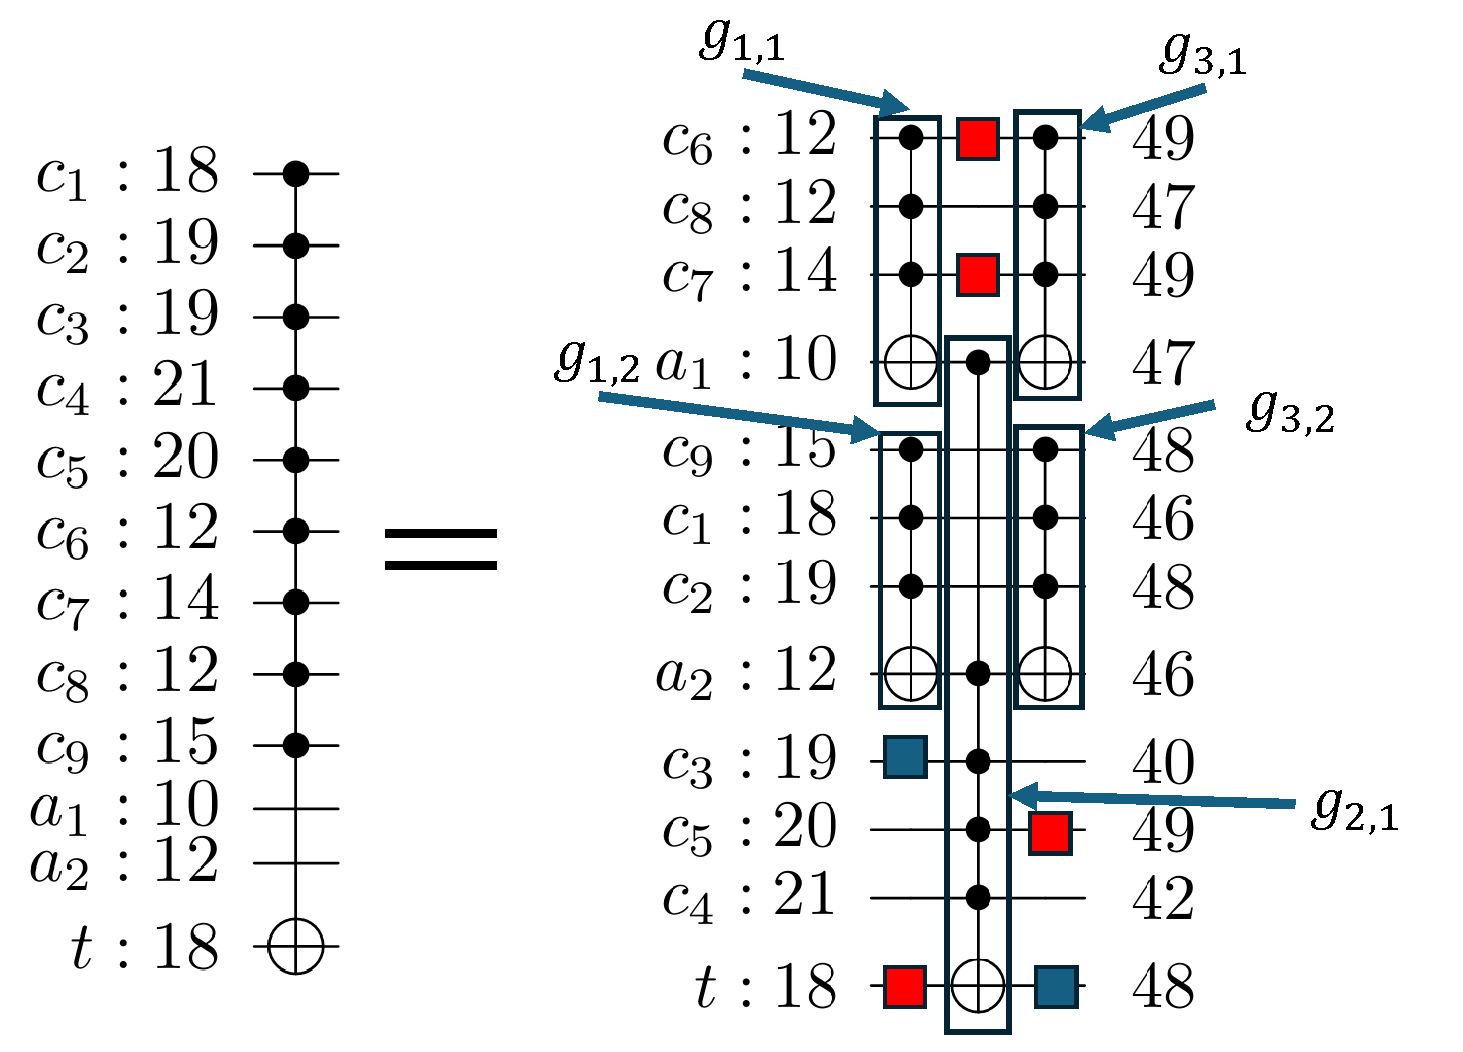
\includegraphics[width=10cm]{img/niemann_proposed.pdf}

\caption{An example of decomposing an MCT gate with $c=9$ using two auxiliary bits with a value of 0,
taking into account the T-depth for each bit, and method~4.}

\label{niemann_proposed}

\end{figure}

Figure ~\ref{niemann_proposed} shows an example of decomposing an MCT gate with $c=9$ using two auxiliary bits with a value of 0,
taking into account the T-depth for each bit, and method~4.
In Figure~\ref{niemann_proposed},
the control bits of the MCT gate before decomposition are $C=\{c_{1},\dots, c_{9}\}$, and the target bit is $t$.

The auxiliary bits with a value of 0 are $CA=\{a_{1}, a_{2}\}$.

First, the number of control bits of the MCT gate at each stage is calculated using method~4, as shown in equation~\ref{eq:niemann_ctrl_gutairei}.

\begin{equation}\label{eq:niemann_ctrl_gutairei}
\begin{pmatrix}

3 & 3 \\

5 & \\
\end{pmatrix}
\end{equation}
The bits that make up each gate are determined according to the number of control bits in equation~\ref{eq:niemann_ctrl_gutairei}.

First, determine the bits that make up the gates $g_{1,1} and g_{1,2}$ in the first to second stages.

When the control bits are selected from $C$ in ascending order of T-depth,
the control bits of the gates in the first stage are $C_{1,1}=\{c_{6}, c_{8}, c_{7}\}$ and $C_{1,2}=\{c_{9}, c_{1}, c_{2}\}$, respectively.

The selected control bits are $C$Then, the target bits for the first-stage gate are selected in ascending order of T-depth, which are $a_{1}$ and $a_{2}$.
The selected auxiliary bit with a value of 0 is added to $C$ and deleted from $CA$.
After determining the bits that make up the first-stage gates $g_{1,1} and g_{1,2}$,
a set $A$ of bits not used in $g_{1,1} and g_{1,2}$ is obtained.
At this time, $A=\{c_{3}, c_{5}, c_{4}, t\}$.
Of these bits, $c_{3} and c_{5}$ are used as auxiliary bits in ascending order of T-depth, $g_{1,1} and g_{1,2}$ are decomposed, and the T-depth is updated.
Next, the bits that make up the second-stage gate $g_{2,1}$ are determined.
Since the gates in the second stage are the central gates,
the control bits are the remaining $C=\{a_{1},a_{2}, c_{3},c_{5},c_{4}\}$,
and the target bit is $t$.
In this way, the bits that make up $g_{1,1}, g_{1,2}, and g_{2,1}$ are determined.
After determining the bits that make up these gates,
the MCT gates are placed in the order of equation~\ref{eq:niemann_gates},
which results in the decomposition of the right side of Figure~\ref{niemann_proposed}.
\par
\bout{Finally, the gates on the right side of Figure~\ref{niemann_proposed} are decomposed
according to Algorithm~\ref{alg:method4_placement_decomp}.
First, decompose the gates $g_{1,1} and g_{1,2}$ in the first stage.
$g_{1,1}$ is decomposed using the bit $t$ filled in red as the auxiliary bit.

$g_{1,2}$ is decomposed using the bit $c_{3}$ filled in blue as the auxiliary bit.

Next, from the result of the decomposition of $g_{1,1} and g_{1,2}$,
$g_{2,1}$ is decomposed using the bits $c_{6} and c_{7}$ filled in red as the auxiliary bits.

Finally, from the result of the decomposition of $g_{2,1}$,
$g_{3,1} and g_{3,2}$ are decomposed using $c_{5} and t$ as the auxiliary bits, respectively.

When all gates are decomposed in this way, the maximum T-depth is 49. }
% Write on the diagram which auxiliary bits were selected.

\begin{comment}
In the proposed method,
the placement and decomposition of the MCT gates after decomposition are determined according to the number of control bits of the MCT gates in each stage obtained by method 4.
Algorithm~\ref{} shows how to determine the placement and decomposition of the MCT gates in each stage.
\begin{algorithm}[tbp]
\caption{Placement and decomposition of method 3 considering T-depth for each bit}
\label{alg:method3_placement_decomp}
\begin{algorithmic}[1]
\Require MCT gate before decomposition $g=(C,t)$
\Require 2D array $CntList$ showing the number of control bits of MCT gates in each stage obtained by method 4
\Require List of bits with value 0 $CA$
\Require List of bits with indefinite value $DA$
\Require T-depth of each bit
\Ensure circuit after decomposition $OC$
\ForEach{$v$ in $CntList$}
\State $n$: Number of elements of $v$
\State $g_{1},\dots, g_{n}$: MCT gate to be placed
\State $C_{1},\dots ,C_{n}$: Set of control bits of each MCT gate
\State $t_{1},\dots ,t_{n}$: Target bits for each MCT gate
\ForEach{$c$ in $v$ with index $i$}
\For{$j=1$ to $c$}
\State $C_{i}$: Add the bit with the smallest T-depth of $C$
\State $C$: Delete the bit with the smallest T-depth
\EndFor
\State $t_{i}$: Add the bit with the smallest T-depth of $CA$
\State $CA$: Delete the bit with the smallest T-depth
\EndFor
\State $g_{1},\dots ,g_{n}$: Decompose the bits considering the T-depth of each bit so that the same auxiliary bits are not used
\State $OC$: Add decomposition of $g_{1},\dots g_{n}$
\State $OC$: Recalculate T-depth
\State $t_{1},\dots, t_{n}$: Add $C$
\EndFor
\end{algorithmic}
\end{algorithm}
\end{comment}
\subsection{Decomposition in reverse order}
In this section, we explain the decomposition of MCT gates in reverse order.

\begin{figure}[tbp]

\centering

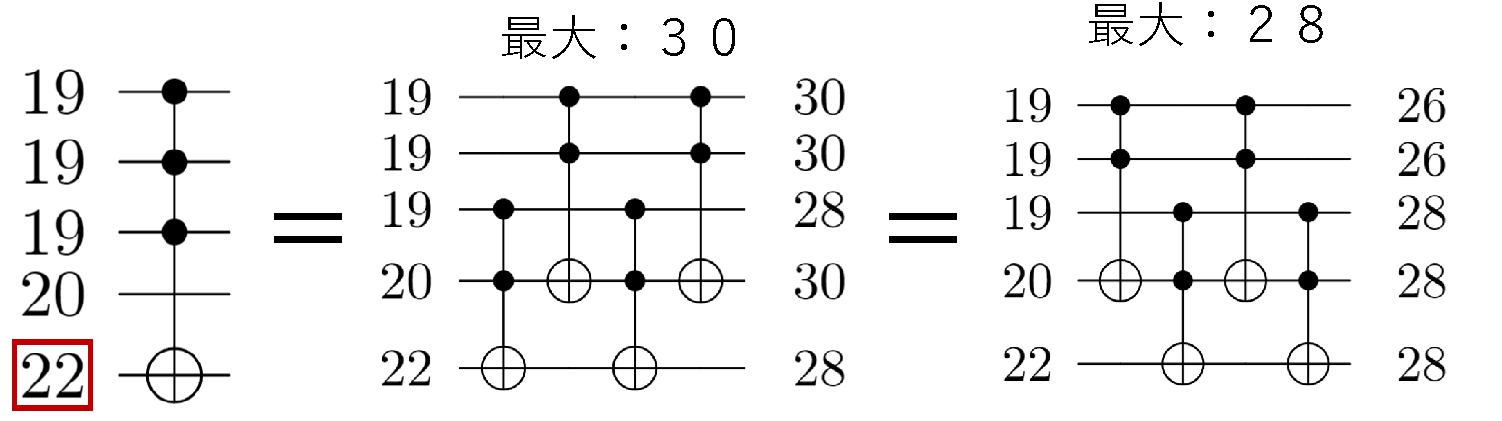
\includegraphics[width=10cm]{img/reverse_mct.pdf}

\caption{Decomposition of an MCT gate with 3 control bits and its decomposition in reverse order}

\label{reverse}

\end{figure}

\par
As shown in Figure~\ref{reverse},
if the T-depth of the target bit is the largest among the auxiliary bits used for the decomposition and the bits that make up the MCT gate to be decomposed,
the T-depth can be reduced by decomposing the MCT gate in reverse order.

The decomposition in the center of Figure~\ref{reverse}
shows the case where the MCT gate on the left side is decomposed in the order of method 1.

On the other hand, the decomposition on the right side shows the case where the MCT gate on the left side is decomposed in the reverse order to the decomposition of method 1.

In the decomposition of the central example, the target bit is always used in the leftmost MCT gate, so the T-depth cannot be reduced.

For this reason, if the T-depth of the target bit is the largest, the T-depth can be reduced by decomposing in reverse order.

In the example in Figure~\ref{reverse}, the maximum T-depth is reduced by 2 by decomposing the MCT gate in reverse order.

\par
To decompose the MCT gate in reverse order using method 1, it is necessary to arrange them in the reverse order of equation~\ref{eq:toffoli_haiti}.

Therefore, it is necessary to use the bits with the smallest T-depth in the order of $g_{2},\dots,g_{c-1},g_{1}$.

The $c$ control bits of the MCT gate before decomposition are rearranged in order of smallest T-depth to be $c_{1},\dots,c_{c}$.
Let $C_{1},\dots,C_{c-1}$ be the set of control bits for $g_{1},\dots,g_{c-1}$.

Let $a_{1},\dots,a_{c-2}$ be the set of $c-2$ undefined auxiliary bits rearranged in ascending order of T-depth.

The method for determining the bits that make up $g_{1},\dots,g_{c-1}$ is shown below.

\begin{enumerate}[Step 1]

\item Let $a_{1}$ be the target bit for $g_{2}$.

\item Add $a_{2},\dots,a_{c-2},a_{1}$ to $C_{2}\dots,C_{c-2},C_{1}$ one by one in order.

\item Add $c_{1}, \dots , and c_{c-3}$ to $C_{2}, \dots , and C_{c-2}$, in that order.
\item Add $c_{c-2} and c_{c-1}$ to $C_{c-1}$.
\item Add $c_{c}$ and $a_{1}$ to $C_{1}$.
\item Let the target bits of $g_{3}, \dots , and g_{c-2}$ be $a_{2}, \dots , and a_{c-3}$, respectively, in that order.
\item Let the target bit of $g_{1}$ be $t$.
\end{enumerate}
After determining the bits that make up $g_{1},\dots, g_{c-1}$,
by arranging them in the reverse order of equation~\ref{eq:toffoli_haiti},
the decomposition of method 1 can be performed in the reverse order.
\par
For method~2, by decomposing in the reverse order, the target bit can be used\bout{later}.
By arranging the four MCT gates $g_{1},\dots, g_{4}$ and the four $C\omega S$ gates in the reverse order, the decomposition in the reverse order can be performed.
The bit with an indefinite value used in the decomposition is $a$.
Even when the four $C\omega S$ gates are decomposed in the reverse order, $a$ remains the control bit and $t$ remains the target bit.
When decomposing in the reverse order, MCT gates are placed from the left in the order of $g_{4}, \dots, g_{1}$, so it is necessary to place bits with small T-depth in $g_{4}, g_{2}$.

Therefore, $C_{2}, C_{1}$ are the sets of control bits for $g_{1}, g_{2}$,
and $C_{1}, C_{2}$ are determined according to equation~\ref{eq:method2bunkatu}.

Once the bits that make up each gate are determined,

by repeating the decomposition and placement in the order of $g_{4}, C\omega S, g_{3}, C\omega S, \dots , g_{1}, C\omega S$,
the decomposition in the reverse order of method~2 can be achieved.

\par
To decompose method 3 in the reverse order,
it is necessary to place the MCT gates decomposed in the reverse order of equation~\ref{eq:bakerhaiti}.
Therefore, it is necessary to arrange the bits with the smallest T-depth in the order of $g_{2}, \dots, g_{m+1}, g_{1}$.

Let $A$ be the set of $m$ auxiliary bits used for decomposition.

Let $N_{1}, \dots, N_{m+1}$ be the number of control bits for each MCT gate $g_{1}, \dots, g_{m+1}$ after decomposition,

obtained by method 3.

Let $C_{1}, \dots, C_{m+1}$ be the set of control bits for $g_{1}, \dots, g_{m+1}$.

Let $t_{1}, \dots, t_{m+1}$ be the target bits for $g_{1}, \dots, g_{m+1}$.

The bits that make up $g_{1},\dots, and g_{m+1}$ are determined according to the following procedure.
\begin{enumerate}[Step 1]
\item Determine the bits that make up $g_{2}$.
\begin{enumerate}
\item Move the element with the smallest T-depth from $A$ to $C_{2}$.
\item Move the element with the smallest T-depth from $A$ to $t_{2}$.
\item Move the element with the smallest T-depth from $C$ to $g_{2}$.
\end{enumerate}
\item Determine the bits that make up $g_{3},\dots, and g_{m+1}$.
\begin{enumerate}
\item Let $i=3$.
\item Move the element with the smallest T-depth from $A$ to $C_{i}$.
\item From $C$ to $N_{i}$ so that $|C_{i}|=N_{i}$.Move elements in ascending order of T-depth.
\item Let $t_{i}$ be the element of $A$ moved to $C_{i-1}$.
\end{enumerate}
\item Determine the bits that make up $g_{1}$.
\begin{enumerate}
\item Add $t_{2}$ to $C_{1}$.
\item Move the remaining elements of $C$ to $C_{1}$.
\item Let $t_{1}$ be $t$.
\end{enumerate}
\end{enumerate}
By using this procedure to determine the bits that make up $g_{1},\dots, and g_{m+1}$, and then arranging the gates in the reverse order of equation~\ref{eq:bakerhaiti},
and decomposing, method 3 can also be decomposed in the reverse order.

As for method 4, since the decomposition is symmetric, there is no change in the T-depth even if the decomposition is performed in the reverse order.
% Methods 2 and 3 are explained separately.
\subsection{Decomposition method using beam search considering subsequent gates}
This section explains the method of decomposing MCT gates using beam search, taking into account subsequent gates.

Figure~\ref{select_ancilla_tdepth} shows the change in T-depth due to the selection of auxiliary bits for two MCT gates $g_{1} and g_{2}$.
The example in the center of Figure~\ref{select_ancilla_tdepth} shows an example in which $g_{1}$ selects the auxiliary bit with the smallest T-depth, which is filled in red, for decomposition, and $g_{2}$ selects the bit with the smallest T-depth, which is filled in blue, based on the result of the decomposition of $g_{1}$.
In the example on the right side of Figure~\ref{select_ancilla_tdepth},
$g_{1}$ selects the auxiliary bit with a T-depth of 41 (filled in red) and decomposes it,
while $g_{2}$ receives the result of the decomposition of $g_{1}$ and selects the bit with the smallest T-depth (filled in blue).
In the example in the center of Figure~\ref{select_ancilla_tdepth},
the maximum T-depth is 58,
while in the example on the right side,
the maximum T-depth is 53.
\begin{figure}[tbp]
\centering
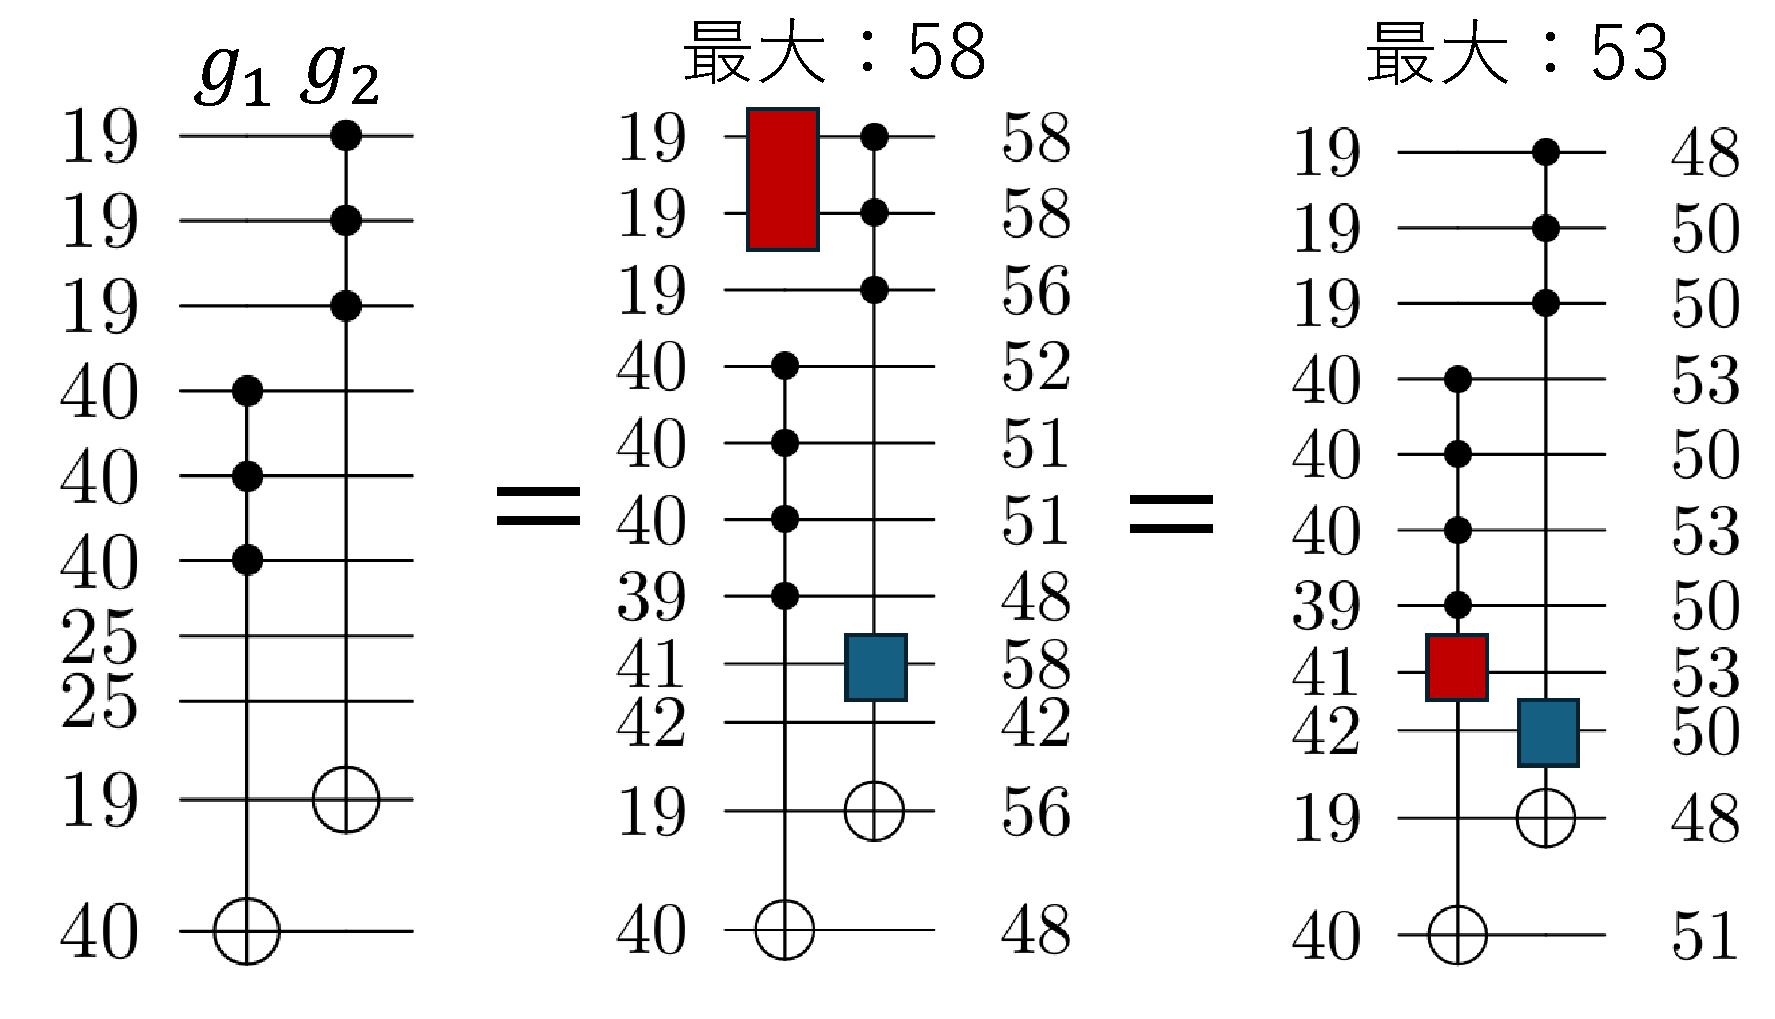
\includegraphics[width=10cm]{img/select_ancilla_biit_tdepth.pdf}
\caption{Example of change in T-depth by selecting auxiliary bits for two MCT gates}
\label{select_ancilla_tdepth}
\end{figure}
As in the central example of Figure~\ref{bad_consider_tdepth},
if a bit with a small T-depth is selected greedily,
the T-depth may worsen when decomposing the \bout{successor} gate.
For this reason, it is necessary to decompose the MCT gate considering the \bout{successor} gate of the gate to be decomposed.
\par
When decomposing MCT gates considering the T-depth for each bit,
the T-depth of each bit changes depending on the result of the decomposition of the MCT gate.
Therefore, a tree is constructed by setting the evaluation value of each node as the maximum T-depth,
and treating the decomposition of each MCT gate as a transition.
The optimal decomposition can be found by exhaustively searching this tree.
However, if a full search is performed, the computational complexity will be enormous as the number of quantum bits and the number of MCT gates to be decomposed increase.

For this reason, we use beam search \cite{bisiani1992beam} to limit the search range to a predetermined number of candidates,
and perform the search while keeping the computational complexity to a realistic level.

Here, we also limit the enumeration of the decompositions of each MCT gate.

To enumerate all the decompositions, we must enumerate all the combinations of the selection of the auxiliary bits.

An MCT gate with $c$ control bits can select $1$ to $c-2$ auxiliary bits with undefined values.

If the number of usable auxiliary bits with undefined values is $m$,
there are $\sum_{i = 1}^{c-2} {}_mC_{i}$ ways to select the auxiliary bits with undefined values.

When the number of quantum bits in the circuit and the number of control bits in the MCT gates that make up the circuit increase,
it is difficult to enumerate all the selections of the auxiliary bits,
so we limit the number of transitions by using the specified decomposition as the transition.
The specified decomposition is as follows.
\begin{enumerate}[(1)]
\item Select 1 to $c-2$ auxiliary bits with undefined values in ascending order of T-depth
\item Select 1 to $c-2$ auxiliary bits with 0 values in ascending order of T-depth
\item Select 1 to $c-2$ bits with undefined values from the bits not used by the gate immediately following the gate performing the decomposition in ascending order of T-depth.
\item Decomposition in reverse order of these decompositions
\end{enumerate}
\par
The pseudo code for beam search is shown in Algorithm~\ref{alg:mct_beam}, where the decomposition of MCT gates is the transition and the maximum T-depth after the decomposition is the evaluation value.
Figure~\ref{mct_beam} shows how the decomposition of $g_{1}$ in Figure~\ref{select_ancilla_tdepth} is determined according to Algorithm~\ref{alg:mct_beam}.

The search width in Figure~\ref{mct_beam} is 3, and the search depth is 2.

For simplicity, the decomposition in reverse order is not enumerated.

First, in Figure~\ref{mct_beam},

the decomposition of $g_{1}$ is enumerated \rout{$D_{1},\dots, D_{4}$. }

The maximum T-depth of the circuit obtained from the decomposition $D_{1},\dots,D_{4}$ is set as the evaluation value of the node.

The nodes are sorted in ascending order of evaluation value,

and the decomposition of the next gate $g_{2}$ is enumerated from the top three nodes.

T-depth is calculated from the result of the decomposition of $g_{2}$,
and the first transition of the node with the smallest evaluation value is determined as the decomposition of $g_{1}$.

In this example, $D_{3}$ is determined as the decomposition of $g_{1}$.

\begin{figure}[tbp]

\centering

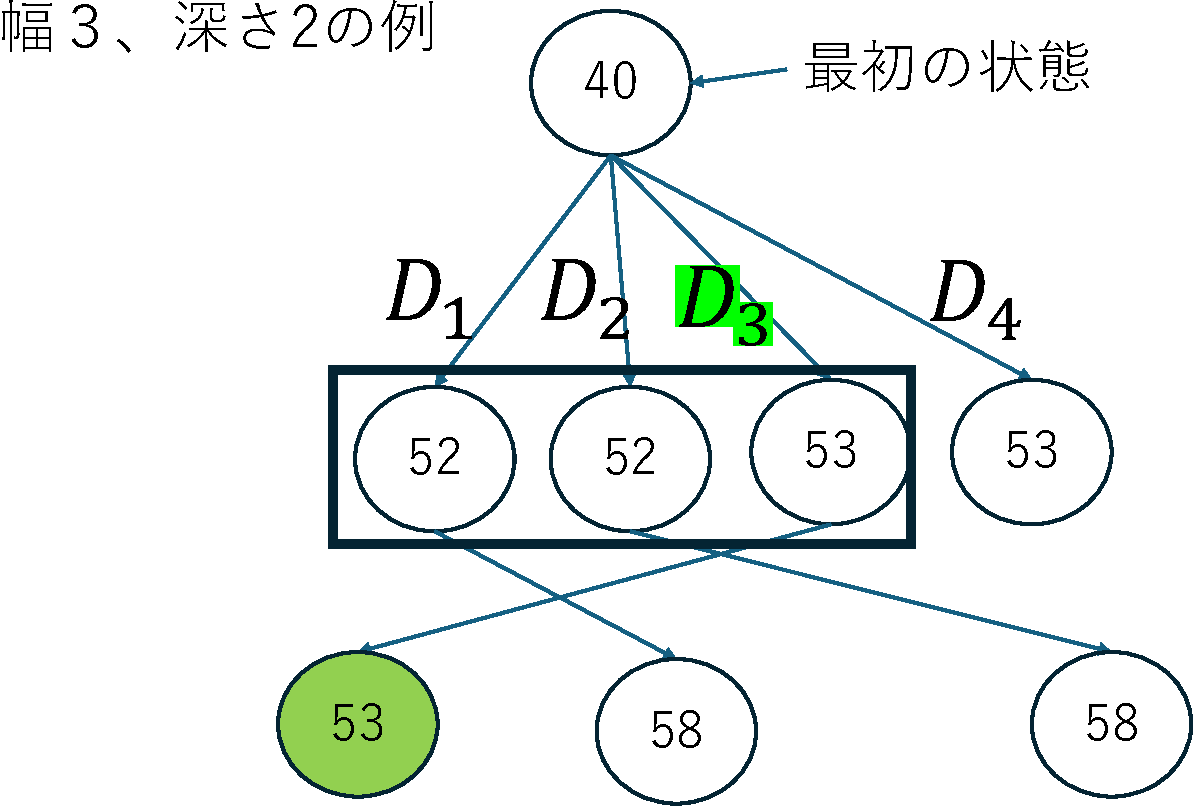
\includegraphics[width=8cm]{img/mct_beam.pdf}

\caption{Figure~\ref{select_ancilla_tdepth} shows how the decomposition of $g_{1}$ is determined according to Algorithm~\ref{alg:mct_beam}}

\label{mct_beam}

\end{figure}

In the proposed method, for a circuit composed of MCT gates, the decomposition is determined gate by gate
based on Algrorithm~\ref{alg:mct_beam}, and all gates are decomposed.

% Should I give a concrete example? The example in the figure is not very good.

\begin{comment}
Figure~\ref{mct_beam} shows how a beam search with a search depth of 2 and width of 3 is used,

Figure~\ref{bad_consider_tdepth} shows how the decomposition of the MCT gate is determined taking into account subsequent gates.
\begin{figure}[tbp]
\centering
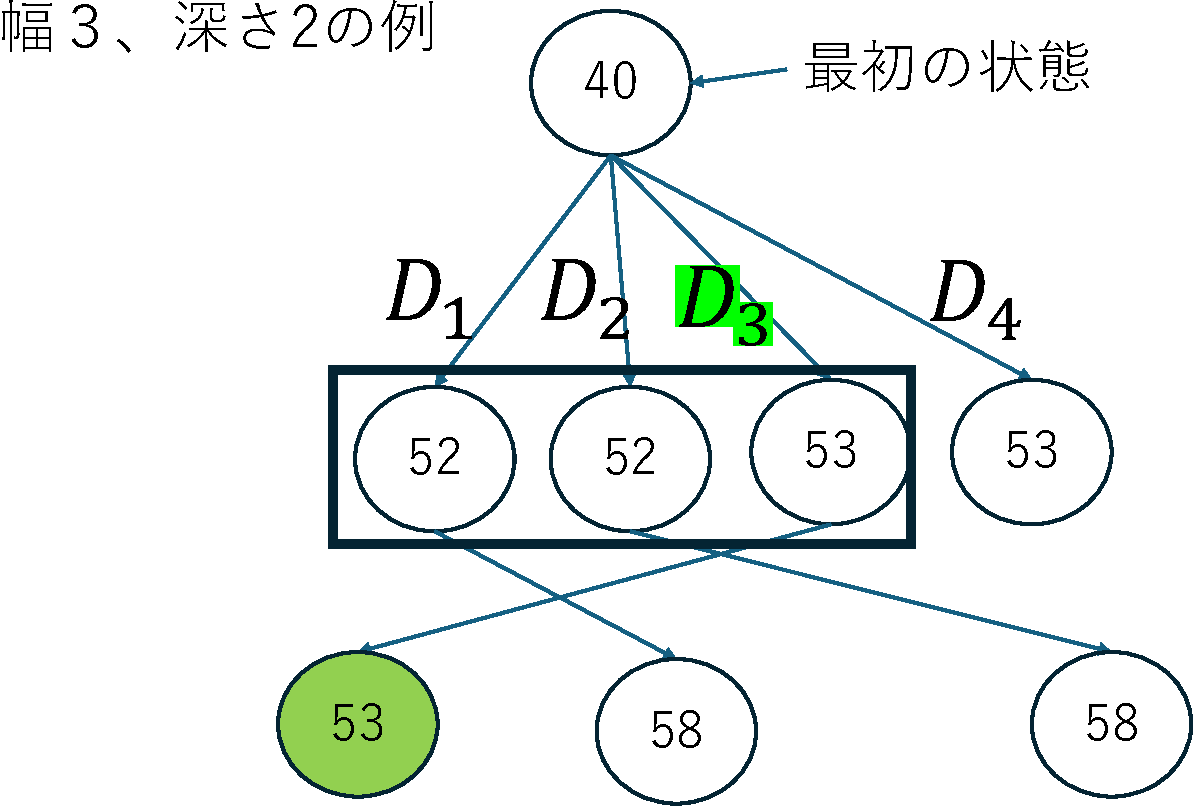
\includegraphics[width=10cm]{img/mct_beam.pdf}
\caption{Example of change in T-depth by selecting auxiliary bits for two MCT gates}
\label{mct_beam}
\end{figure}
\end{comment}

\begin{algorithm}[tbp]
\caption{Pseudocode for beam search with maximum T-depth as evaluation value}
\label{alg:mct_beam}
\begin{algorithmic}[1]
\Require $state$: (maximum T-depth, T-depth per bit, MCT gate to be decomposed)
\Require $legal\_actions$: Function to enumerate decompositions of MCT gates and return the state before the next gate decomposition
\Require $depth$: Depth to search
\Require $width$: Width to search
\State $best\_decomp$: Best candidate
\State $candidate\_list$ List of search candidates, prioritized queue
\State $candidate\_list.push(state)$
\For{$1,..,depth$}
\State $next\_candidate\_list$ List of next search candidates, prioritized queue
\For{$1,..,width$}
\If{If $candidate\_list$ is empty}
\State break
\EndIf
\State $now\_state \Leftarrow candidate\_list.pop()$ Extract the best value of the search candidate and pop it
\State $next\_candidate\_list.push(legal\_actions(now\_state))$ Add the transition from the current state to the list of next search candidates
\EndFor
\State $candidate\_list \Leftarrow next\_candidate\_list$ Update the list of search candidates
\State $best\_decomp \Leftarrow candidate\_list.top()$ Update the best candidate
\EndFor
\State \Return Return the first transition of $best\_decomp$
\end{algorithmic}
\end{algorithm}
